\documentclass[12pt, a4paper]{article}

% ── Codificación y lenguaje ───────────────────────────────────────────────────
\usepackage[T1]{fontenc}
\usepackage[utf8]{inputenc}
\usepackage[spanish]{babel}

% ── Márgenes ─────────────────────────────────────────────────────────────────
\usepackage[top=2.5cm, bottom=2.5cm, left=3cm, right=3cm]{geometry}

% ── Gráficos y figuras ────────────────────────────────────────────────────────
\usepackage{graphicx}
\usepackage{float}

% ── Tablas ────────────────────────────────────────────────────────────────────
\usepackage{booktabs}

% ── Código fuente ─────────────────────────────────────────────────────────────
\usepackage{listings}
\usepackage{xcolor}

\definecolor{codegray}{rgb}{0.95, 0.95, 0.95}
\definecolor{codecomment}{rgb}{0.4, 0.4, 0.4}
\definecolor{codestring}{rgb}{0.13, 0.5, 0.11}
\definecolor{codekeyword}{rgb}{0.13, 0.13, 0.8}

\lstset{
    language=C++,
    basicstyle=\ttfamily\small,
    backgroundcolor=\color{codegray},
    keywordstyle=\color{codekeyword}\bfseries,
    commentstyle=\color{codecomment}\itshape,
    stringstyle=\color{codestring},
    numbers=left,
    numberstyle=\tiny\color{gray},
    numbersep=8pt,
    breaklines=true,
    breakatwhitespace=false,
    frame=single,
    rulecolor=\color{gray!40},
    tabsize=4,
    captionpos=b,
    showstringspaces=false,
    inputencoding=utf8,
    extendedchars=true,
    literate=
        {á}{{\'a}}1 {é}{{\'e}}1 {í}{{\'i}}1 {ó}{{\'o}}1 {ú}{{\'u}}1
        {Á}{{\'A}}1 {É}{{\'E}}1 {Í}{{\'I}}1 {Ó}{{\'O}}1 {Ú}{{\'U}}1
        {ñ}{{\~n}}1 {Ñ}{{\~N}}1
}

% ── Hipervínculos ─────────────────────────────────────────────────────────────
\usepackage{hyperref}
\hypersetup{
    colorlinks=true,
    linkcolor=black,
    urlcolor=blue,
    citecolor=black
}

% ── Otros ────────────────────────────────────────────────────────────────────
\usepackage{parskip}
\setlength{\parskip}{6pt}

% ─────────────────────────────────────────────────────────────────────────────

\begin{document}

% ════════════════════════════════════════════════════════════════════════════
%  PORTADA
% ════════════════════════════════════════════════════════════════════════════
\begin{titlepage}
    \centering
    \vspace*{2cm}

    {\LARGE \textbf{Universidad Nacional de La Plata} \par}
    \vspace{0.4cm}
    {\large Facultad de Ingeniería \par}

    \vspace{2cm}
    \rule{\linewidth}{0.5pt}
    \vspace{0.4cm}

    {\Huge \textbf{Trabajo Práctico IoT} \par}
    \vspace{0.4cm}
    {\Large Estación de Monitoreo Ambiental \par}

    \vspace{0.4cm}
    \rule{\linewidth}{0.5pt}

    \vspace{2.5cm}

    {\large
    \begin{tabular}{ll}
        \textbf{Apellido y nombre:} & \underline{\hspace{6cm}} \\[1em]
        \textbf{Legajo:}            & \underline{\hspace{6cm}} \\
    \end{tabular}
    \par}

    \vfill

    {\large La Plata, Argentina \par}
    \vspace{0.3cm}
    {\large \today \par}
\end{titlepage}

% ════════════════════════════════════════════════════════════════════════════
%  ÍNDICE
% ════════════════════════════════════════════════════════════════════════════
\tableofcontents
\newpage

% ════════════════════════════════════════════════════════════════════════════
%  1. INTRODUCCIÓN
% ════════════════════════════════════════════════════════════════════════════
\section{Introducción}

El objetivo de este trabajo práctico es implementar una estación de monitoreo ambiental
utilizando tecnologías de Internet de las Cosas (IoT). La idea central es construir un
sistema completo que abarque desde la adquisición de datos en un dispositivo embebido
hasta la visualización de esos datos en un dashboard web, pasando por transporte,
procesamiento y almacenamiento.

Para eso se utilizó un microcontrolador ESP32 con un sensor DHT22, capaz de medir
temperatura y humedad relativa. Los datos se transmiten a través del protocolo MQTT,
se procesan con Node-RED, se almacenan en InfluxDB y finalmente se grafican en Grafana.

Cada componente del sistema tiene una responsabilidad clara, y la comunicación entre
ellos está desacoplada, lo que permite modificar o reemplazar partes sin afectar al
resto del sistema.

% ════════════════════════════════════════════════════════════════════════════
%  2. ARQUITECTURA DEL SISTEMA
% ════════════════════════════════════════════════════════════════════════════
\section{Arquitectura del sistema}

El sistema está compuesto por los siguientes componentes, conectados en cadena:

\begin{enumerate}
    \item \textbf{ESP32 + DHT22:} dispositivo de campo que lee temperatura y humedad
          y publica los datos vía MQTT.
    \item \textbf{Mosquitto:} broker MQTT que recibe los mensajes del ESP32 y los
          distribuye a los suscriptores.
    \item \textbf{Node-RED:} recibe los mensajes MQTT, los parsea y los reenvía a
          InfluxDB.
    \item \textbf{InfluxDB:} base de datos de series temporales donde se persisten
          las mediciones.
    \item \textbf{Grafana:} herramienta de visualización que consulta InfluxDB y
          muestra los datos en un dashboard.
\end{enumerate}

La figura~\ref{fig:arquitectura} ilustra el flujo general de la información a lo
largo del sistema.

% CAPTURA A INSERTAR: diagrama general del flujo ESP32 -> MQTT -> Node-RED -> InfluxDB -> Grafana
\begin{figure}[H]
    \centering
    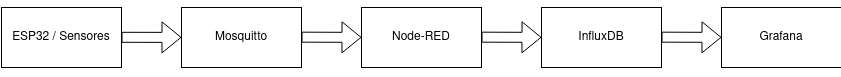
\includegraphics[width=0.9\textwidth]{imagenes/arquitectura.png}
    \caption{Diagrama general de la arquitectura del sistema.}
    \label{fig:arquitectura}
\end{figure}

A modo de referencia, el flujo de datos puede representarse así:

\begin{center}
\ttfamily
ESP32 + DHT22 $\longrightarrow$ Mosquitto (MQTT) $\longrightarrow$ Node-RED
$\longrightarrow$ InfluxDB $\longrightarrow$ Grafana
\end{center}

Mosquitto, Node-RED, InfluxDB y Grafana corren como contenedores Docker en la misma
máquina. El ESP32 se conecta a la red local y se comunica con el broker por IP.

% ════════════════════════════════════════════════════════════════════════════
%  3. ESP32 Y SENSOR DHT22
% ════════════════════════════════════════════════════════════════════════════
\section{ESP32 y sensor DHT22}

\subsection{Rol del ESP32}

El ESP32 actúa como el nodo de campo del sistema. Su trabajo es leer el sensor,
armar un mensaje con los datos y publicarlo en el broker MQTT. Es la única parte
del sistema que interactúa directamente con el hardware físico.

El firmware se desarrolló con PlatformIO desde Visual Studio Code, usando el
framework Arduino. Las bibliotecas utilizadas son:

\begin{itemize}
    \item \texttt{knolleary/PubSubClient} (v2.8): cliente MQTT liviano para Arduino.
    \item \texttt{adafruit/DHT sensor library} (v1.4.6): lectura del sensor DHT22.
    \item \texttt{adafruit/Adafruit Unified Sensor} (v1.1.14): dependencia de la anterior.
\end{itemize}

\subsection{Sensor DHT22}

El DHT22 es un sensor digital de temperatura y humedad relativa. Devuelve lecturas
con una resolución de $0{,}1\,^\circ\text{C}$ y $0{,}1\,\%$ de humedad,
respectivamente. Su interfaz es de un único cable de datos (single-wire), y se
comunica con el microcontrolador a través de un protocolo propio. En el proyecto, la
línea de datos está conectada al GPIO~18 del ESP32.

El sensor se inicializa en \texttt{setup()} y se lee en el \texttt{loop()} cada
5000\,ms. Si la lectura devuelve \texttt{NaN} (lo que ocurre ante un error de
comunicación o cableado incorrecto), se descarta y se imprime un aviso por el monitor
serial sin publicar ningún dato al broker.

\subsection{Configuración del firmware}

Los parámetros de conexión (SSID, contraseña WiFi, IP del broker, pin del sensor e
intervalo de publicación) están definidos en el archivo \texttt{include/config.h}.
Este archivo no se sube al repositorio; en su lugar existe \texttt{config.example.h}
como plantilla.

\subsection{Fragmento principal del firmware}

El código~\ref{lst:firmware} muestra la función \texttt{loop()} junto con la lógica
de lectura y publicación. La parte de reconexión WiFi y MQTT se maneja en funciones
auxiliares separadas (\texttt{connectWiFi()} y \texttt{connectMQTT()}).

\begin{lstlisting}[language=C++, caption={Función \texttt{loop()} del firmware ESP32.}, label={lst:firmware}]
void loop() {
    if (WiFi.status() != WL_CONNECTED) {
        Serial.println("[WiFi] Conexion perdida. Reconectando...");
        connectWiFi();
    }

    if (!mqttClient.connected()) {
        connectMQTT();
    }
    mqttClient.loop();

    unsigned long now = millis();
    if (now - lastPublish >= PUBLISH_INTERVAL_MS) {
        lastPublish = now;

        float temperature = dht.readTemperature();
        float humidity    = dht.readHumidity();

        if (isnan(temperature) || isnan(humidity)) {
            Serial.println("[DHT22] ERROR: Lectura invalida (NaN).");
            return;
        }

        Serial.printf("[DHT22] Temperatura: %.1f C  Humedad: %.1f%%\n",
                      temperature, humidity);

        char payload[128];
        snprintf(payload, sizeof(payload),
            "{\"temperature\":%.1f,\"humidity\":%.1f,"
            "\"source\":\"esp32-dht22\",\"uptime_ms\":%lu}",
            temperature, humidity, now);

        bool ok = mqttClient.publish(MQTT_TOPIC, payload);
        if (ok) {
            Serial.println("[MQTT] Publicacion exitosa.");
        } else {
            Serial.println("[MQTT] ERROR: Fallo al publicar.");
        }
    }
}
\end{lstlisting}

El JSON que se publica tiene la forma:

\begin{lstlisting}[language={}, caption={Ejemplo de payload publicado por el ESP32.}]
{"temperature":23.5,"humidity":61.0,"source":"esp32-dht22","uptime_ms":45132}
\end{lstlisting}

El campo \texttt{source} sirve para identificar el origen de los datos en caso de
que haya más dispositivos publicando en el mismo broker. El campo \texttt{uptime\_ms}
indica cuántos milisegundos lleva encendido el ESP32, lo que puede ser útil para
detectar reinicios inesperados.

% ════════════════════════════════════════════════════════════════════════════
%  4. MQTT Y MOSQUITTO
% ════════════════════════════════════════════════════════════════════════════
\section{MQTT y Mosquitto}

MQTT (\textit{Message Queuing Telemetry Transport}) es un protocolo de mensajería
liviano, diseñado para dispositivos con recursos limitados y redes con ancho de banda
reducido. Funciona con un modelo \textit{publish/subscribe}: los productores publican
mensajes en \textit{tópicos}, y los consumidores que están suscriptos a esos tópicos
los reciben automáticamente. El intermediario que gestiona esta distribución es el
\textit{broker}.

En este proyecto:

\begin{itemize}
    \item El \textbf{ESP32} actúa como \textit{publisher}: publica las mediciones en
          el tópico \texttt{sensor/ambiente} con QoS~0.
    \item \textbf{Mosquitto} actúa como broker, escuchando en el puerto \texttt{1883}.
    \item \textbf{Node-RED} actúa como \textit{subscriber}: está suscripto al mismo
          tópico y recibe cada mensaje que el ESP32 publica.
\end{itemize}

Una ventaja de este modelo es que el ESP32 no necesita saber quién va a consumir los
datos. Si se quisiera agregar otro suscriptor (por ejemplo, una aplicación de
alertas), bastaría con suscribirlo al mismo tópico sin tocar el firmware.

Mosquitto corre en un contenedor Docker y está configurado para aceptar conexiones
anónimas, sin autenticación, ya que el sistema se ejecuta en una red local controlada.
Añadir autenticación sería una mejora natural en una etapa posterior.

% ════════════════════════════════════════════════════════════════════════════
%  5. NODE-RED
% ════════════════════════════════════════════════════════════════════════════
\section{Node-RED}

Node-RED es una herramienta de programación visual orientada a flujos. Permite
conectar servicios y dispositivos mediante nodos que se encadenan en un editor web.
En este proyecto funciona como el middleware entre MQTT e InfluxDB.

El flujo implementado tiene la siguiente estructura:

\begin{enumerate}
    \item \textbf{MQTT In} (\texttt{sensor/ambiente}): se suscribe al tópico y recibe
          cada mensaje publicado por el ESP32.
    \item \textbf{JSON}: convierte el payload de texto plano a un objeto JavaScript.
    \item \textbf{Function} (\textit{Preparar para InfluxDB}): extrae los campos
          \texttt{temperature} y \texttt{humidity}, valida que no sean \texttt{NaN}
          y construye el objeto que espera el nodo de salida de InfluxDB.
    \item \textbf{InfluxDB Out}: escribe los datos en el bucket \texttt{iot}, dentro
          de la medición \texttt{ambiente}.
\end{enumerate}

El flujo también incluye nodos de debug para inspeccionar el payload en distintas
etapas, y un nodo \texttt{catch} que captura errores del nodo de escritura y los
muestra en la consola lateral. Esto facilita detectar problemas de conexión o datos
mal formateados.

% CAPTURA A INSERTAR: flujo de Node-RED mostrando mqtt in -> json/function -> influxdb out
\begin{figure}[H]
    \centering
    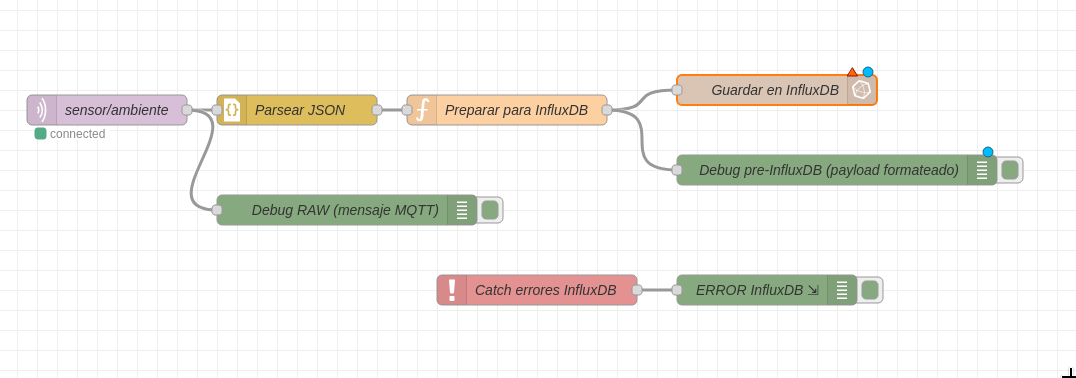
\includegraphics[width=0.9\textwidth]{imagenes/nodered-flujo.png}
    \caption{Flujo de Node-RED: recepción MQTT, parseo JSON y escritura en InfluxDB.}
    \label{fig:nodered}
\end{figure}

% ════════════════════════════════════════════════════════════════════════════
%  6. INFLUXDB
% ════════════════════════════════════════════════════════════════════════════
\section{InfluxDB}

InfluxDB es una base de datos diseñada específicamente para series temporales.
A diferencia de una base relacional clásica, cada punto de datos lleva un
\textit{timestamp} implícito y el motor está optimizado para escrituras frecuentes
y consultas sobre rangos de tiempo. Estas características la hacen especialmente
adecuada para aplicaciones IoT, donde los sensores generan datos continuamente.

En este proyecto se usa InfluxDB~2.x. La configuración relevante es:

\begin{itemize}
    \item \textbf{Organización:} \texttt{iot-org}
    \item \textbf{Bucket:} \texttt{iot}
    \item \textbf{Medición:} \texttt{ambiente}
    \item \textbf{Campos:} \texttt{temperature} (°C) y \texttt{humidity} (\%)
\end{itemize}

La tabla~\ref{tab:influx} muestra un ejemplo representativo de cómo se almacenan
los datos.

\begin{table}[H]
    \centering
    \caption{Ejemplo de datos almacenados en InfluxDB (medición \texttt{ambiente}).}
    \label{tab:influx}
    \begin{tabular}{@{}lcc@{}}
        \toprule
        \textbf{Timestamp (UTC)} & \textbf{temperature (°C)} & \textbf{humidity (\%)} \\
        \midrule
        2024-11-10T14:00:00Z & 23.5 & 61.0 \\
        2024-11-10T14:00:05Z & 23.6 & 60.8 \\
        2024-11-10T14:00:10Z & 23.6 & 61.1 \\
        2024-11-10T14:00:15Z & 23.5 & 61.3 \\
        \bottomrule
    \end{tabular}
\end{table}

Dado que el ESP32 publica cada 5\,segundos, en una hora se acumulan aproximadamente
720~filas por campo. InfluxDB maneja este volumen sin inconvenientes y permite
consultar rangos amplios de manera eficiente.

% ════════════════════════════════════════════════════════════════════════════
%  7. GRAFANA
% ════════════════════════════════════════════════════════════════════════════
\section{Grafana}

Grafana es una plataforma de visualización y análisis de datos. Permite construir
dashboards con gráficos, tablas y otros paneles, conectándose a distintas fuentes de
datos. En este proyecto se usa para visualizar las mediciones almacenadas en InfluxDB.

La fuente de datos está configurada mediante aprovisionamiento automático: al
levantar los contenedores, Grafana ya tiene la conexión a InfluxDB lista sin
necesidad de configurarla manualmente desde la interfaz. El datasource apunta a
\texttt{http://influxdb:8086} usando el token de autenticación definido en la
configuración de InfluxDB.

El dashboard incluye dos paneles de tipo \textit{Time series}:

\begin{itemize}
    \item \textbf{Temperatura}: muestra la evolución de la temperatura en el tiempo,
          con unidad \texttt{°C}.
    \item \textbf{Humedad}: muestra la evolución de la humedad relativa, con
          unidad~\texttt{\%}.
\end{itemize}

Ambos paneles muestran estadísticas de mínimo, máximo y promedio en la leyenda.
El rango temporal se puede ajustar libremente desde los controles del dashboard.

Las consultas están escritas en Flux (el lenguaje de consultas de InfluxDB~2.x).
La consulta para temperatura, a modo de ejemplo, es:

\begin{lstlisting}[language={}, caption={Consulta Flux para graficar la temperatura en Grafana.}]
from(bucket: "iot")
  |> range(start: v.timeRangeStart, stop: v.timeRangeStop)
  |> filter(fn: (r) => r["_measurement"] == "ambiente")
  |> filter(fn: (r) => r["_field"] == "temperature")
\end{lstlisting}

La consulta de humedad es análoga, cambiando el valor del filtro de \texttt{\_field}
a \texttt{"humidity"}.

% CAPTURA A INSERTAR: dashboard de Grafana mostrando gráficos de temperatura y humedad
\begin{figure}[H]
    \centering
    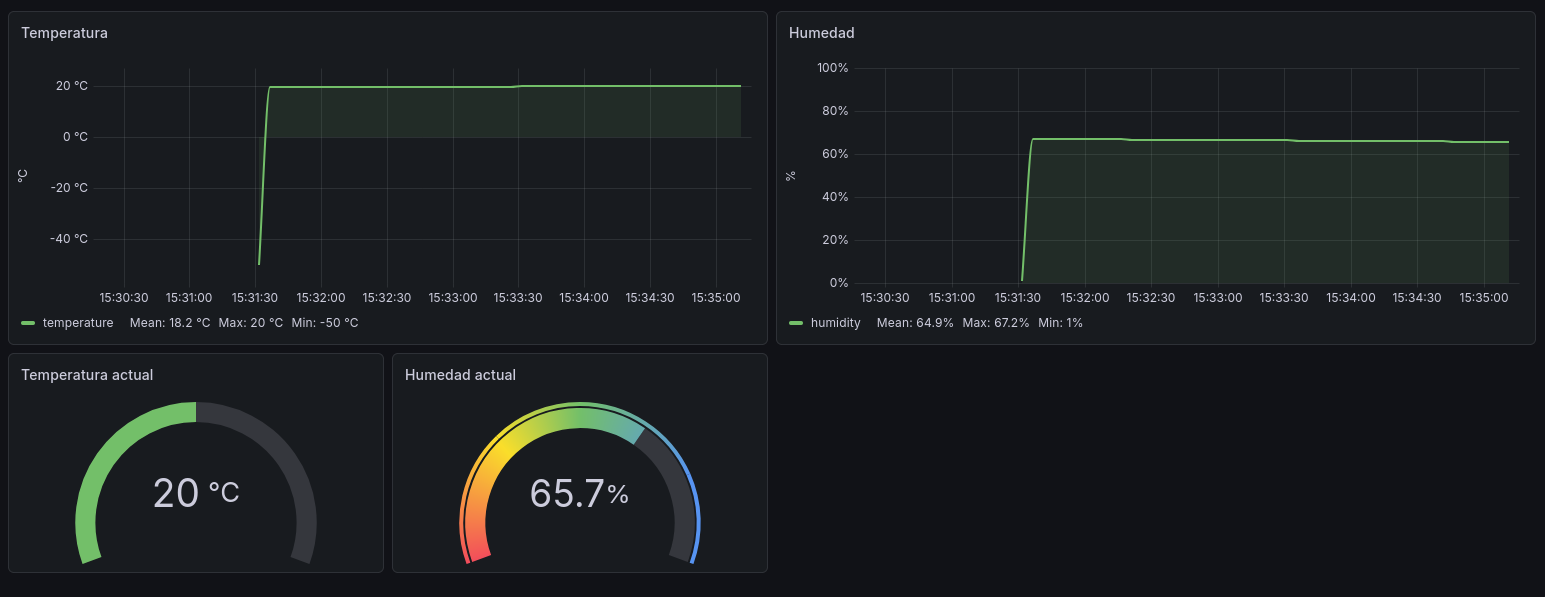
\includegraphics[width=0.9\textwidth]{imagenes/grafana-dashboard.png}
    \caption{Dashboard de Grafana con las mediciones de temperatura y humedad.}
    \label{fig:grafana}
\end{figure}

% ════════════════════════════════════════════════════════════════════════════
%  8. INFRAESTRUCTURA Y EJECUCIÓN
% ════════════════════════════════════════════════════════════════════════════
\section{Infraestructura y ejecución}

\subsection{Servicios en Docker}

Los cuatro servicios del backend (Mosquitto, Node-RED, InfluxDB y Grafana) se
levantan juntos con Docker Compose. Cada uno corre en su propio contenedor con
la red y los volúmenes necesarios para persistir datos entre reinicios.

Para iniciar el sistema completo:

\begin{lstlisting}[language=bash, caption={Inicio y verificación de los contenedores.}]
docker compose up -d
docker compose ps
\end{lstlisting}

Una vez en ejecución, las interfaces web de cada servicio son accesibles desde
el navegador:

\begin{itemize}
    \item \textbf{Node-RED:} \texttt{http://localhost:1880}
    \item \textbf{InfluxDB:} \texttt{http://localhost:8086}
    \item \textbf{Grafana:} \texttt{http://localhost:3000}
\end{itemize}

\subsection{Firmware del ESP32}

El firmware se compila y se carga al ESP32 desde PlatformIO. Los pasos son:

\begin{enumerate}
    \item Copiar \texttt{include/config.example.h} a \texttt{include/config.h} y
          completar con los valores reales (SSID, contraseña WiFi, IP del broker,
          pin del sensor).
    \item Compilar y flashear con PlatformIO (botón \textit{Upload} en VS Code,
          o \texttt{pio run --target upload} desde la terminal).
    \item Verificar el comportamiento en el monitor serial a 115200\,baud.
\end{enumerate}

El archivo \texttt{platformio.ini} define el entorno de compilación: plataforma
\texttt{espressif32}, placa \texttt{esp32dev}, framework \texttt{arduino} y
velocidad del monitor serial en 115200.

% ════════════════════════════════════════════════════════════════════════════
%  9. PRUEBAS REALIZADAS
% ════════════════════════════════════════════════════════════════════════════
\section{Pruebas realizadas}

Se verificó el funcionamiento de cada etapa del sistema de forma independiente antes
de validar el flujo completo extremo a extremo.

\subsection{Lectura del sensor y publicación MQTT}

Con el monitor serial abierto a 115200\,baud se observó que el ESP32 imprime la
temperatura y humedad cada 5\,segundos y confirma la publicación en el tópico
\texttt{sensor/ambiente}.

% CAPTURA A INSERTAR: monitor serial del ESP32 mostrando temperatura, humedad y publicación MQTT
\begin{figure}[H]
    \centering
    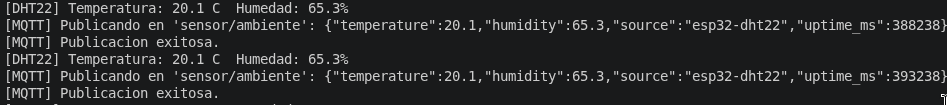
\includegraphics[width=0.9\textwidth]{imagenes/monitor-serial.png}
    \caption{Monitor serial mostrando lecturas del DHT22 y confirmación de publicación MQTT.}
    \label{fig:serial}
\end{figure}

\subsection{Recepción de mensajes en Node-RED}

El panel de debug de Node-RED mostró los payloads MQTT recibidos en tiempo real,
lo que permitió verificar que el broker estaba distribuyendo los mensajes
correctamente y que el parseo JSON funcionaba sin errores.

% CAPTURA A INSERTAR: consola o debug de Node-RED mostrando el payload MQTT recibido
\begin{figure}[H]
    \centering
    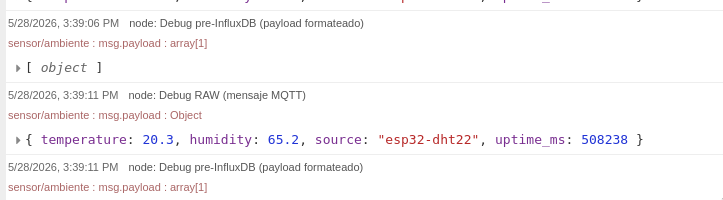
\includegraphics[width=0.9\textwidth]{imagenes/mqtt-debug.png}
    \caption{Panel de debug de Node-RED con los mensajes recibidos desde el ESP32.}
    \label{fig:mqtt-debug}
\end{figure}

\subsection{Almacenamiento en InfluxDB}

Desde la interfaz web de InfluxDB se consultó el bucket \texttt{iot} y se verificó
que los datos se estaban escribiendo con el timestamp correcto y los campos
\texttt{temperature} y \texttt{humidity} con los valores esperados.

\subsection{Visualización en Grafana}

Una vez con datos en InfluxDB, el dashboard de Grafana mostró las curvas de
temperatura y humedad actualizándose a medida que el ESP32 publicaba nuevas
mediciones. Se ajustó el rango temporal del panel para ver la evolución en los
últimos minutos y verificar la continuidad de los datos.

% ════════════════════════════════════════════════════════════════════════════
%  10. CONCLUSIONES Y POSIBLES MEJORAS
% ════════════════════════════════════════════════════════════════════════════
\section{Conclusiones y posibles mejoras}

\subsection{Conclusiones}

El trabajo práctico permitió construir e integrar un sistema IoT completo, desde la
lectura de un sensor físico hasta la visualización de los datos en un dashboard web.
Cada componente del sistema tiene una responsabilidad bien delimitada, y la
comunicación entre ellos se realiza a través de interfaces estándar (MQTT, HTTP,
Flux), lo que facilita el mantenimiento y la extensión del sistema.

A lo largo del desarrollo se entendió en la práctica el modelo
\textit{publish/subscribe} de MQTT, el rol de Node-RED como capa de integración, y
cómo InfluxDB está optimizado para manejar el tipo de datos que genera un sensor
que mide continuamente.

La arquitectura elegida es escalable: agregar un sensor adicional implicaría
básicamente publicar en un nuevo tópico MQTT (o en el mismo con campos extra) sin
modificar ninguna otra parte del sistema.

\subsection{Posibles mejoras}

\begin{itemize}
    \item \textbf{Más sensores:} incorporar sensores de calidad del aire (CO\textsubscript{2},
          partículas), luminosidad o presión barométrica.
    \item \textbf{Autenticación MQTT:} configurar usuario y contraseña en Mosquitto
          para evitar conexiones no autorizadas.
    \item \textbf{Credenciales:} cambiar el token de InfluxDB y la contraseña de
          Grafana por valores distintos a los valores por defecto.
    \item \textbf{Almacenamiento local en el ESP32:} si se pierde la conexión WiFi
          o MQTT, guardar temporalmente las lecturas en memoria y reenviarlas cuando
          se restablezca la conexión.
    \item \textbf{Alertas en Grafana:} configurar alertas que notifiquen cuando la
          temperatura o la humedad superen umbrales definidos.
    \item \textbf{MQTT sobre TLS:} cifrar el canal de comunicación entre el ESP32
          y el broker, especialmente si el sistema se expone fuera de la red local.
\end{itemize}

\end{document}
